\begin{problem}{파티}
	{standard input}{standard output}
	{3 seconds}{128 megabytes}{}
	
	
범수는 파티를 열려고 한다. 당연히 그는 파티가 잘 되었으면 좋겠다고 생각한다. 그리고 범수는 초대하는 모든 손님들이 서로를 알고 있으면 파티가 성공 할 것이라고 확신한다. 그래서 그는 초대하고 싶은 친구 목록을 만드려고 한다.

범수는 $n$명의 친구가 있고, $n$은 3의 배수이다. 운이 좋게도 대부분의 범수의 친구들은 서로를 안다. 그리고 $\frac{2}{3}n$ 명이 파티를 했고, 그 때 서로서로를 아는 사람이 있던 기억이 난다. 하지만 범수는 그 때 술을 마시다가 필름이 끊겨서 그 파티가 잘 기억이 안 난다. 특히, 파티에 누가 있었는지 기억을 못한다. 


범수는 소소하게 $\frac{n}{3}$명으로 파티를 하려고 한다. 범수는 어떻게 친구들을 초대해야 할 지 모르기 때문에 당신에게 도움을 요청했다.

	

	\InputFile
	
	첫째 줄에는 두 개의 정수 범수의 친구 수를 의미하는 $n$과 친구끼리 서로 아는 관계를 표현하는 $m$이 공백 하나로 구분되어 주어진다. ($3 \le n \le 3,000$, $\dfrac{\frac{2}{3}n\left(\frac{2}{3}n-1\right)}{2} \le m \le \dfrac{n(n-1)}{2}$ ) 범수에 친구는 1번부터 $n$번까지 번호가 붙어있다. 다음 $m$개의 줄의 $i$번째 줄에는 $a_i$와 $b_i$가 공백 하나로 구분되어 주어진다. ($1 \le a_i < b_i \le n$) 이것은 친구 $a_i$와 $b_i$가 서로를 안다는 뜻이다. 같은 숫자 쌍은 최대 한 번 입력에 등장한다.
	
	\OutputFile
	
	첫째 줄에 $\frac{n}{3}$개의 숫자를 공백 하나로 구분하여 출력한다. 이 숫자들은 오름차순으로 정렬되어 있어야 한다. 이 숫자는 범수가 파티에 초대할 사람들을 나타내야 한다. 답이 여러개인 경우 아무 답이나 출력해도 좋다.
	\Examples
		
	\begin{example}
	\exmp{
6 10
2 5
1 4
1 5
2 4
1 3
4 5
4 6
3 5
3 4
3 6

	}{%
2 4

	}%
	\end{example}
	
	\Note
	
	\begin{center}
	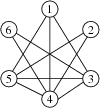
\includegraphics[]{imp.png}
	\end{center}
	
	범수의 친구중 1, 3, 4, 5번 친구는 서로를 안다. 하지만 2, 4 같은 다른 쌍도 정답이 될 수 있다. 정답이 서로 아는 4명중 2명이 아니여도 된다.
	
\end{problem}

